\documentclass[11pt, a4paper]{article}
\usepackage[utf8]{inputenc}
\usepackage[T1]{fontenc}
\usepackage{helvet}
\renewcommand{\familydefault}{\sfdefault}
\usepackage[table]{xcolor}
\definecolor{schoolgreen}{HTML}{92D050}
\usepackage{geometry}
\geometry{landscape, margin=1.5cm, top=4cm, headheight=2.5cm, headsep=0.5cm}
\usepackage{array}
\usepackage{graphicx}
\usepackage{fancyhdr}
\usepackage{longtable}
\usepackage{amssymb}
\pagestyle{fancy}
\fancyhf{}
\fancyhead[L]{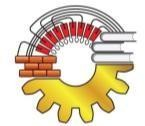
\includegraphics[height=2cm]{../../distritos/4117/templates/logo1.jpg}}
\fancyhead[R]{
\includegraphics[height=2cm]{../../distritos/4117/templates/logo2.jpg}}
\fancyhead[C]{\fontsize{10}{12}\selectfont \textbf{\textit{ESCUELA N.° 4-117 EJÉRCITO DE LOS ANDES \\ DIRECCIÓN DE EDUCACIÓN TÉCNICA Y TRABAJO \\ SECCIÓN V}}}
\renewcommand{\headrulewidth}{0pt}

\begin{document}
\noindent\colorbox{schoolgreen}{\begin{minipage}{\dimexpr\textwidth-2\fboxsep}\centering \textbf{\fontsize{14}{16}\selectfont PLANIFICACIÓN ANUAL 2026}\end{minipage}}

\vspace{1em}
\begin{flushleft}
\textbf{Espacio Curricular:} Termodinámica y Máquinas Térmicas \\
\textbf{Ciclo Lectivo:} 2026 \\
\textbf{Curso:} 5to 2da \\
\textbf{Profesor Responsable:} Ferreyra Gustavo David
\end{flushleft}

\vspace{1em}
\noindent \textbf{FUNDAMENTACIÓN:}
\textit{La Termodinámica es la ciencia que estudia la energía y sus transformaciones, siendo el pilar fundamental para comprender el funcionamiento de motores, calderas y sistemas de refrigeración. Para el Técnico Electromecánico, es crucial dominar los conceptos de calor, trabajo y entropía para optimizar procesos industriales y desarrollar tecnologías energéticamente eficientes. Esta planificación busca vincular la teoría abstracta con la realidad técnica de las máquinas térmicas.}

\vspace{1em}
\noindent \textbf{ACUERDOS DE ÁREA:}
\begin{itemize}
\item Rigurosidad en el uso de unidades del Sistema Internacional (SI).
\item Análisis crítico de la eficiencia energética en los procesos industriales.
\item Integración de simulaciones computacionales para la visualización de ciclos térmicos.
\end{itemize}

\vspace{1em}
\noindent \textbf{CAPACIDADES INSTITUCIONALES:}
\begin{itemize}
\item Comprender y producir textos orales y escritos con eficacia y autonomía.
\item Aplicar conocimientos, habilidades, destrezas, actitudes y valores en la resolución y planteo de situaciones problemáticas con creatividad, eficacia, eficiencia, calidad, seguridad y productividad.
\end{itemize}

\vspace{1em}
\noindent \textbf{CAPACIDADES ESPECÍFICAS DEL ÁREA:}
\begin{itemize}
\item Analizar la transformación de energía térmica en trabajo mecánico.
\item Calcular el rendimiento de máquinas térmicas y ciclos de potencia.
\item Interpretar diagramas termodinámicos (P-V, T-S).
\item Evaluar el impacto ambiental de los sistemas de generación de energía térmica.
\end{itemize}

\vspace{1em}
\begin{longtable}{|p{2.5cm}|p{3cm}|p{4cm}|p{3cm}|p{2.5cm}|p{1.5cm}|p{3cm}|}
\hline
\rowcolor{gray!20} \textbf{Saberes/ Contenidos} & \textbf{Aprendizajes Prioritarios} & \textbf{Estrategias Didácticas} & \textbf{Capacidades Específicas} & \textbf{Recursos} & \textbf{Tiempo} & \textbf{Evaluación} \\
\hline
\multicolumn{7}{|l|}{\textbf{EJE Nº 1: FUNDAMENTOS TÉRMICOS Y SISTEMAS}} \\
\hline
Transmisión de Calor y Sistemas & Comprender los mecanismos de conducción, convección y radiación & Resolución de problemas, uso de termómetros & Análisis conceptual & Termómetros, simuladores & 4 semanas & Pruebas escritas, ejercicios \\
\hline
Primer Principio y Balance Térmico & Aplicar la conservación de la energía en sistemas cerrados & Análisis de balances térmicos & Cálculo termodinámico & Software de simulación & 4 semanas & Informes técnicos, resolución de casos \\
\hline
\multicolumn{7}{|l|}{\textbf{EJE Nº 2: GASES PERFECTOS Y TRANSFORMACIONES}} \\
\hline
Leyes de los Gases y Avogadro & Aplicar la ecuación de estado y la ley de Avogadro & Resolución de problemas, análisis de datos & Cálculo gasométrico & Tablas de gases, simuladores & 4 semanas & Pruebas escritas, ejercicios \\
\hline
Transformaciones Termodinámicas & Analizar procesos isotérmicos, isobáricos e isocóricos & Estudio de diagramas P-V & Interpretación técnica & Software de simulación & 4 semanas & Informes de laboratorio, rúbricas \\
\hline
\multicolumn{7}{|l|}{\textbf{EJE Nº 3: CICLOS, ENTROPÍA Y MÁQUINAS TÉRMICAS}} \\
\hline
Segunda Ley y Entropía & Analizar la irreversibilidad y el concepto de entropía & Estudio de casos, análisis de ciclos & Análisis crítico & Tablas termodinámicas & 4 semanas & Pruebas escritas, defensa oral \\
\hline
Ciclos de Combustión Interna & Comparar los ciclos Otto y Diesel en rendimiento & Análisis de diagramas P-V & Interpretación de ciclos & Simuladores de motores & 6 semanas & Proyecto de análisis de motor, rúbricas \\
\hline
\multicolumn{7}{|l|}{\textbf{EJE Nº 4: PROCESOS DE CAMBIO DE FASE Y REFRIGERACIÓN}} \\
\hline
Vaporización y Ciclo Rankine & Analizar la generación de vapor y potencia térmica & Estudio de diagramas de Mollier & Cálculo de potencia & Tablas de vapor, diagramas & 4 semanas & Informe técnico, resolución de casos \\
\hline
Refrigeración y Laboratorio & Diseñar sistemas de frío y validar experimentalmente & Prácticas de laboratorio, medición de carga & Diseño y aplicación & Manómetros, cámaras frías & 4 semanas & Proyecto de refrigeración, rúbricas \\
\hline
\end{longtable}

\vspace{1em}
\noindent \textbf{PROYECTOS DE ARTICULACIÓN:}
\begin{tabular}{|p{5cm}|p{12cm}|}
\hline
\rowcolor{gray!20} \textbf{Proyecto} & \textbf{Actividades y Temas de Articulación} \\
\hline
Articulación Proyecto Alfabetización & Redacción de un glosario técnico de termodinámica y elaboración de informes sobre la eficiencia energética. \\
\hline
Articulación Proyecto de Matemáticas & Aplicación de integrales y logaritmos para el cálculo de entropía y trabajo en procesos reales. \\
\hline
Articulación Proyecto de Bullyng & Fomento de la cultura de la seguridad y el respeto mutuo en el análisis de riesgos industriales. \\
\hline
\end{tabular}
\end{document}